The time obtained from the raw fitting of the waveform requires corrections in order to account for various crystal-to-crystal time offsets that can result due to time walk and differences in hardware (such as cable lengths). The overall time offset for each crystal can be corrected using the accelerator RF signal, and the time walk can be removed through study of hits and hit energies in a cluster versus that of the seed hit energy. The corrected individual crystal time is shown in Equation~\eqref{eq:toff}.

\begin{equation}
	\label{eq:toff}
	t = t_0 +\Delta t_{RF} + \Delta t_w (E)
\end{equation}

In Equation~\eqref{eq:toff}, $t_0$ is the time calculated from fit to the raw ADC distribution of a crystal, $\Delta t_{RF}$ is the hit time offset with the accelerator RF signal, and $\Delta t_w(E)$ is the energy-dependent time-walk correction. The accelerator has a an intrinsic frequency of 499 MHz, and the RF signal is sampled every 80 signals into Hall B. The RF signal in the hall is readout by two FADC250 channels. The raw waveform of the RF signal is shown in Figure~\ref{Figure:rfFits}. 

\begin{figure}[H]
  \centering
      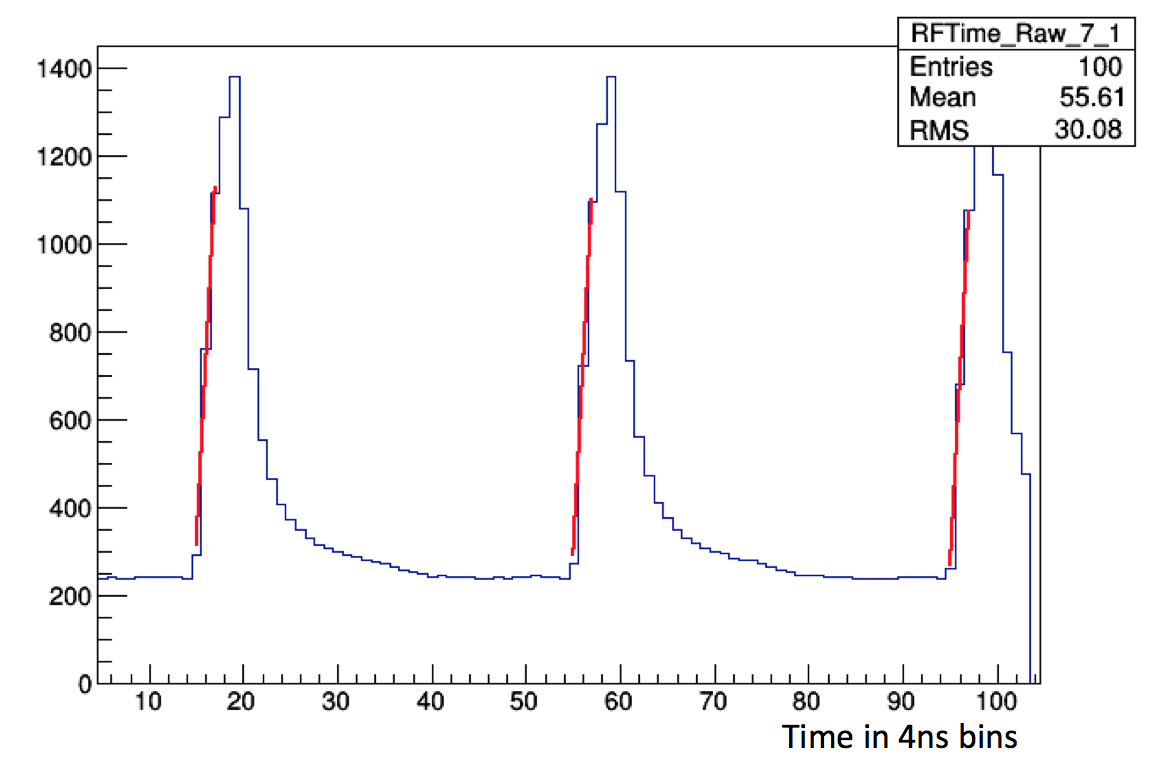
\includegraphics[width=0.7\textwidth]{pics/performance/rfFits.png}
  \caption[Fitted, raw waveform of the RF signal in HPS]{The raw distribution of the RF signal is shown with a straight line fit to the leading edge of the signal.}
  \label{Figure:rfFits}
\end{figure}

The strategy to read off the time from the RF signal was chosen in order to minimize the measured intrinsic resolution of the FADC modules. After identifying the peak bin (4~ns per bin), the pedestal was calculated by
averaging the values in 4 bins occurring at 6 to 9 samples prior to the peak. The threshold used in selecting the fitting points was found by calculating the 1/3 height between the averaged pedestal and the peak. The points for the straight line fit were then chosen as the last point below this threshold and the next two points above the threshold. These points were chosen due to the linear uniformity of the pulse away from the
peak bin. The time that was used from this fit was at the half height between the pedestal and the peak. This combination of parameters minimized the width of the time difference distribution between the RF signals in the two FADC channels as shown in Figure~\ref{Figure:intrTres}. 

\begin{figure}[H]
  \centering
      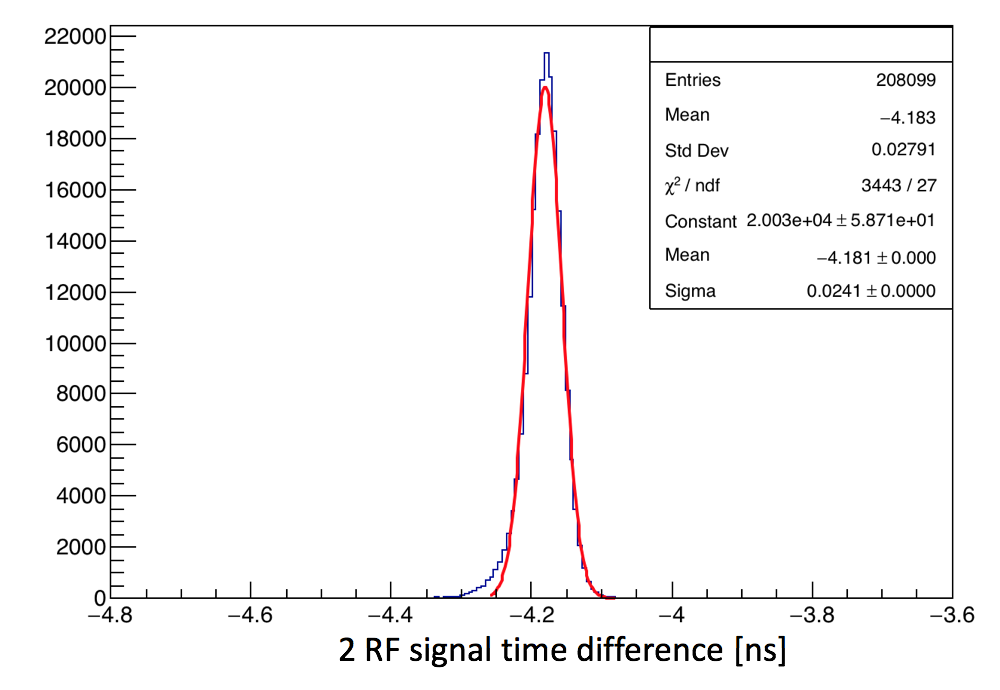
\includegraphics[width=0.7\textwidth]{pics/performance/rfRes.png}
  \caption[FADC intrinsic time resolution]{The intrinsic time resolution of the FADC modules can be obtained by the width of the two RF signal time difference to be approximately 24~ps.}
  \label{Figure:intrTres}
\end{figure}

The internal time resolution of the FADC modules was measured to be approximately 24~ps from the width of the time difference between the two RF signals. The individual crystal module time offsets are measured with respect to the accelerator RF time. For time offsets less than 2~ns, or the time between electron bunches from the accelerator, we calculate the fine time offset per crystal as shown in Equation~\eqref{eq:tfine}.

\begin{equation}
	\label{eq:tfine}
	\Delta t_{fine} = modulo(t_0 - t_{RF} + N\times 2.004, 2.004) - 1.002 \textsf{ ns}
\end{equation}

In Equation~\eqref{eq:tfine}, $t_0$ is the time for the crystal as reported from pulse-fitting, $t_{RF}$ is the reported RF time, and $N$ is an arbitrarily large integer to shift the distribution to all positive values. 2.004~ns pertains to 499~MHz accelerator RF frequency. Before applying Equation~\eqref{eq:tfine}, we observe the beam bunch structure in the time difference between the crystal hits and the RF time in Figure~\ref{Figure:beamBunch}. 

\begin{figure}[H]
  \centering
      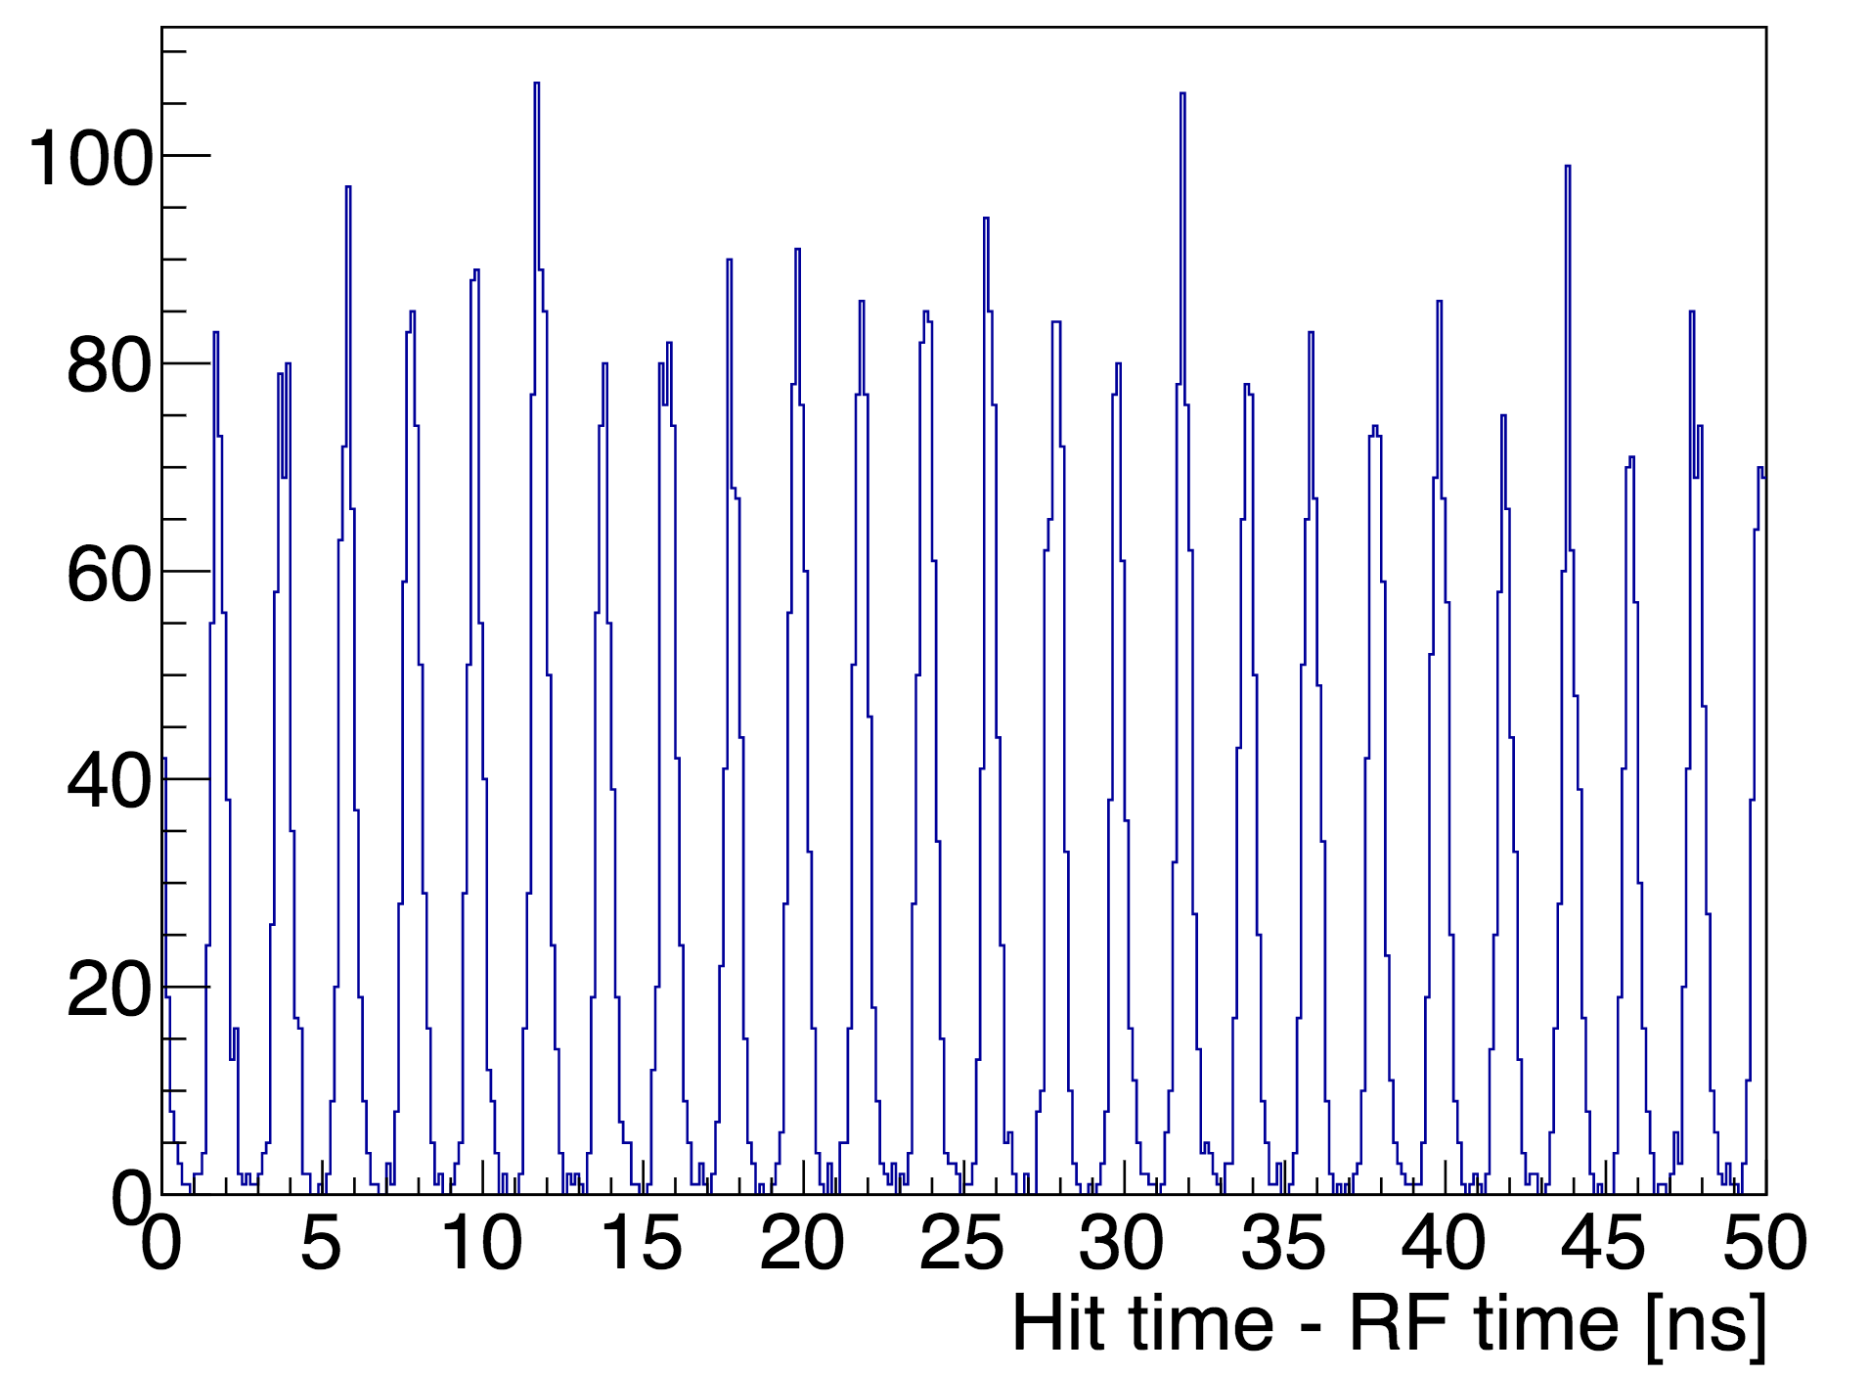
\includegraphics[width=0.7\textwidth]{pics/performance/beamStructure.png}
  \caption[Time difference between ECal hits and RF time]{From the time difference between ECal hits and the RF time, electron beam bunch structure is seen to occur at approximately 2~ns, consistent with known accelerator frequency.}
  \label{Figure:beamBunch}
\end{figure}

By applying Equation~\eqref{eq:tfine} to Figure~\ref{Figure:beamBunch}, we align all of the signals and see the fine offset of each module with respect to the RF time. This technique only shows the offset component that is less than 2~ns and results in all crystals being aligned to the nearest 2$n$~ns, where $n$ is any integer. 


To fully align the crystals, we choose a crystal to align with RF signal at 0, and then align all other crystals with respect to this crystal. Because the primary trigger for HPS is a cluster pairs trigger, we can compare the time difference between clusters to make this correction. The time of the highest energy hit in a cluster was used to set the time for the cluster. Comparison studies exploring the use of an energy-weighted cluster time using the hit times in a cluster found no significant difference due to the seed hit energy dominating the time distribution and producing the same results as if one had used the time from the seed hit only. Well-correlated pairs of clusters were selected by looking for pairs with an energy sum equal to the beam energy and an energy difference of less than 200~MeV. The times for both clusters must have occurred in the 30-70~ns time window for the Engineering Run which was the optimal time window for triggered events. The time difference correction between two pairs of clusters after the fine time offset correction is shown in Figure~\ref{Figure:2clusoffset}.

\begin{figure}[H]
  \centering
      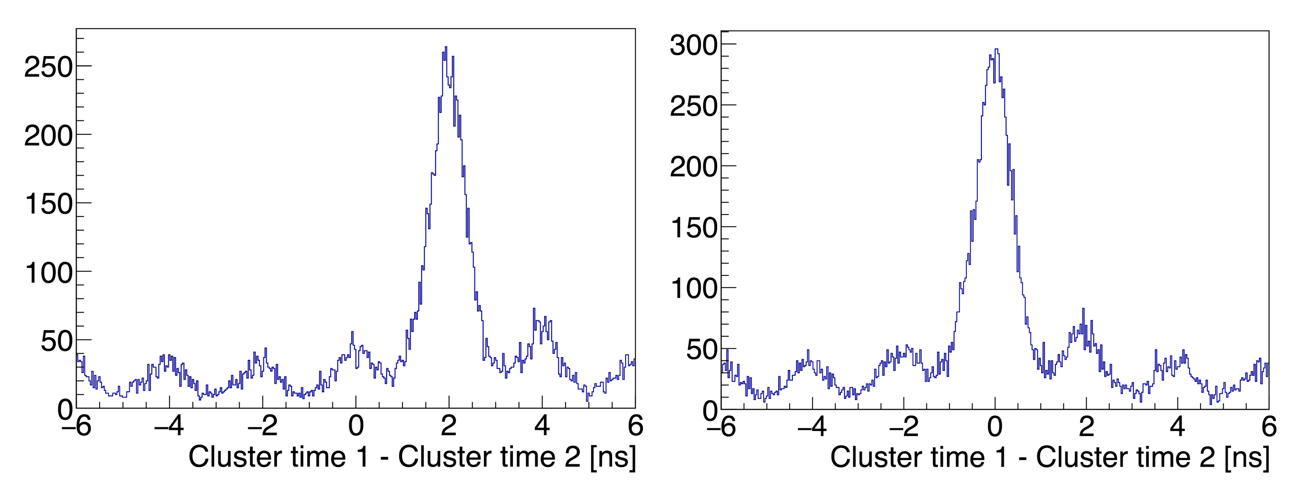
\includegraphics[width=0.9\textwidth]{pics/performance/2clusteroffset.png}
  \caption[Time difference between two clusters after fine offset time correction]{After correcting all clusters with the fine timing offset correction, clusters are aligned to the nearest 2~ns time offset with respect to the RF signal. Shown on the left is a cluster pair that has an overall 2~ns time difference that needs to be accounted for in the final offset with the RF time. The plot on the right shows a different cluster pair with an offset centered at 0.}
  \label{Figure:2clusoffset}
\end{figure}

In Figure~\ref{Figure:2clusoffset}, a large 2~ns offset between a cluster pair is seen on the left prior to this step in the timing correction with respect to the RF signal. A different cluster pair, shown on the right, is seen to have no overall time offset that needs to be accounted for with respect to the RF time. \\
\indent After correcting for the time offsets of all crystals with respect to the RF time, an energy-dependent correction, known as the time walk correction, must be accounted for. Time walk is the time difference of a signal crossing threshold in an ADC due to the finite rise time of the leading edge and the difference in signal amplitudes for particles of different energies. The effect causes particles of lower energy to cross the threshold later in time than particles of higher energy. This effect is not physical and can be removed by studying the time difference between hits in a cluster versus the seed hit as a function of the hit energy. Pulse fitting of the raw signal removes most of the time walk when compared to other methods that can be used to obtain a hit time. In the Engineering Run data, the seed hit was greater than 400 MeV and provided a reasonable threshold against which to compare hit times at lower energies. For the Physics Run data, the time walk correction was able to use a much higher seed hit threshold of 1~GeV, and the energy-dependence could be extended to higher energies. The time walk can be extracted from the comparison of the the hit times within a cluster as shown in Figure~\ref{Figure:hittimeincluster}.

\begin{figure}[H]
  \centering
      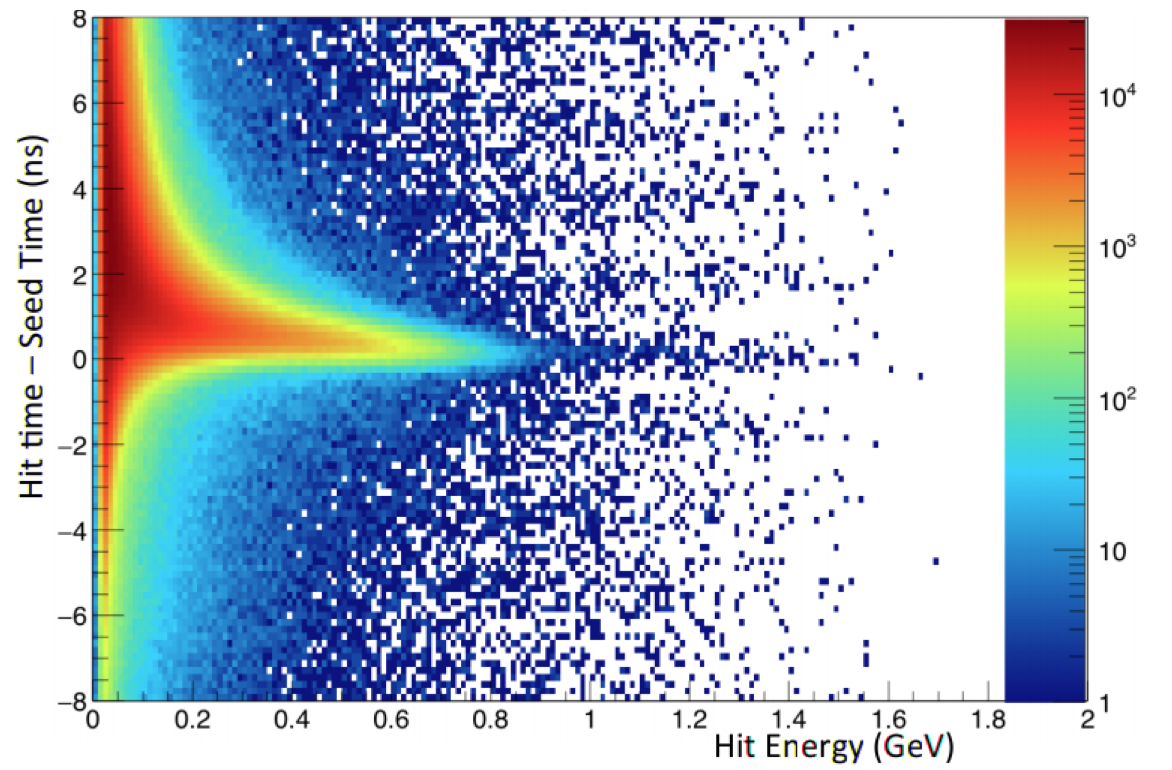
\includegraphics[width=0.7\textwidth]{pics/performance/hittimeincluster.png}
  \caption[Hit times in a cluster versus the hit energy]{The time walk correction for the 2016 data can be extracted from the difference of hit times in a cluster versus the seed hit time as a function of the the hit energy.}
  \label{Figure:hittimeincluster}
\end{figure}

The time walk correction found from the Physics Run data is shown in Figure~\ref{Figure:twalk}. 

\begin{figure}[H]
  \centering
      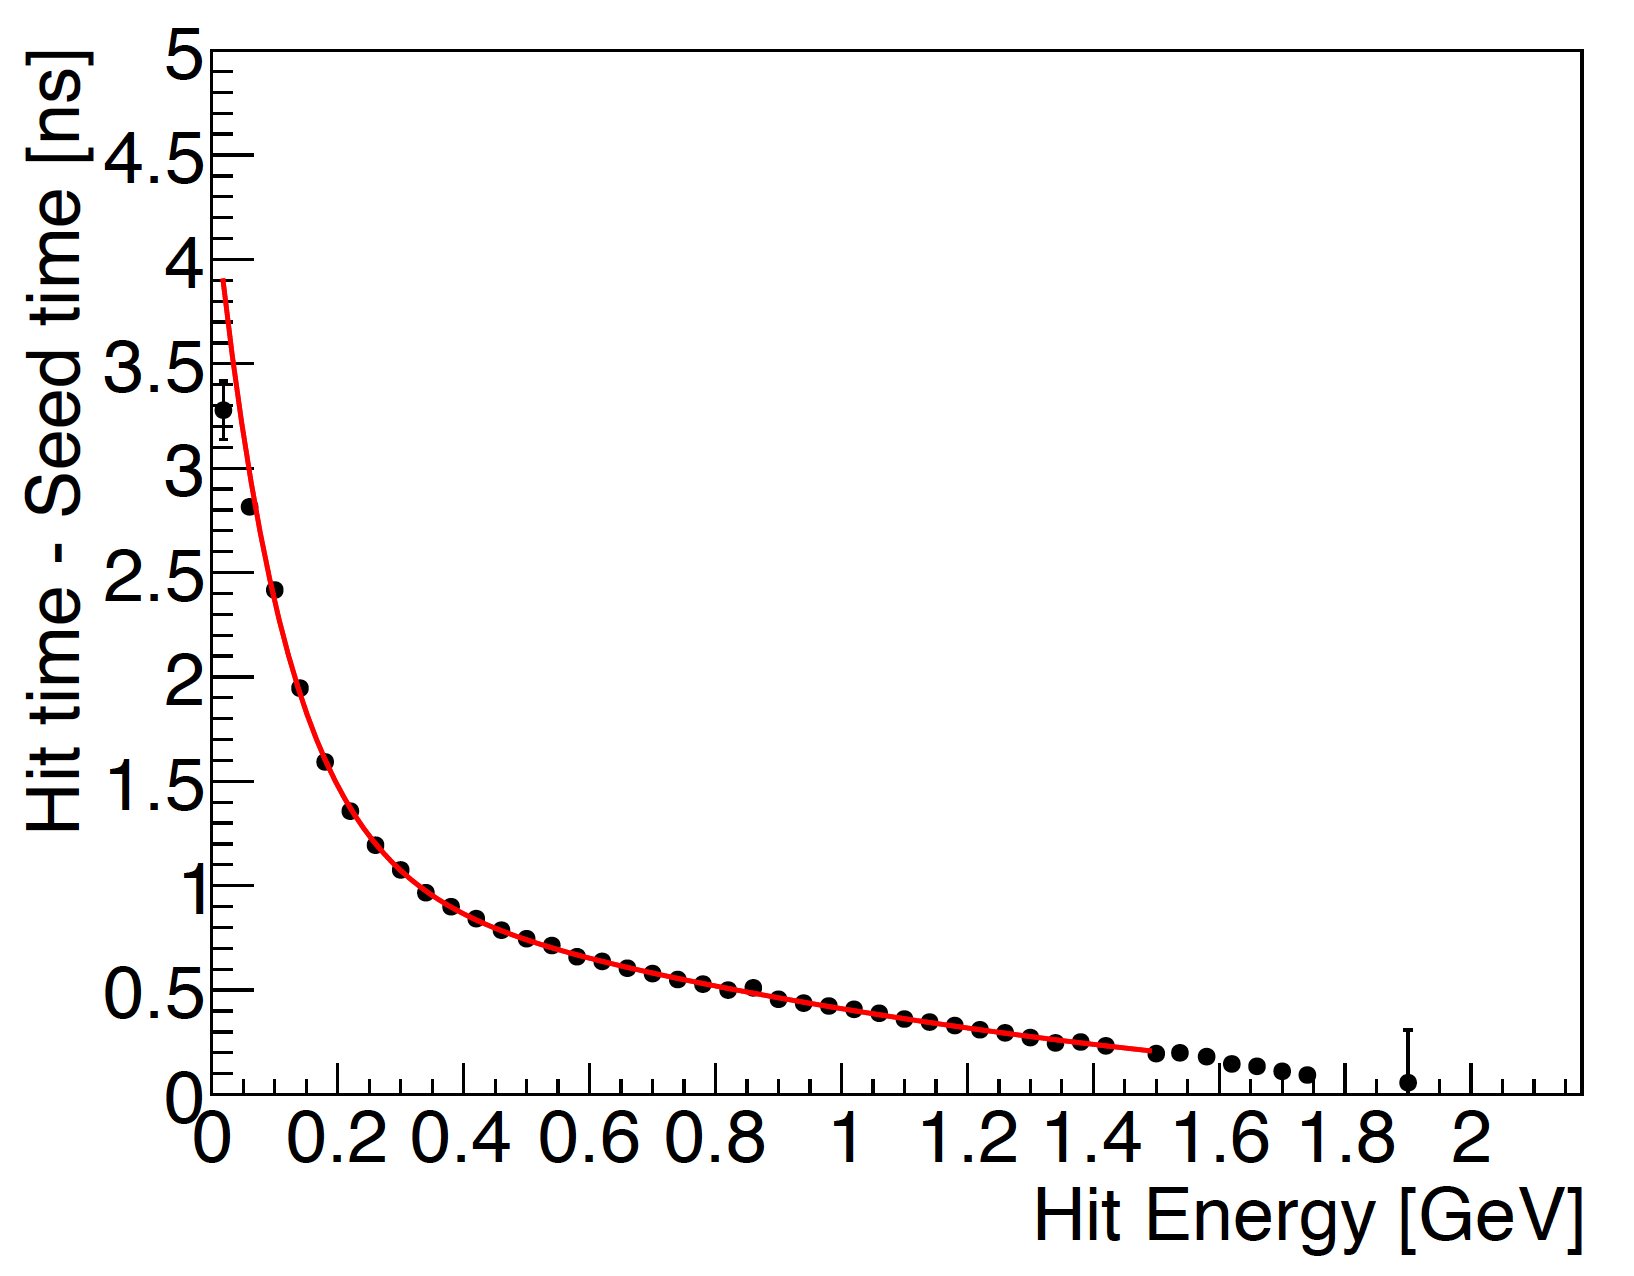
\includegraphics[width=0.6\textwidth]{pics/performance/twalk2016.png}
  \caption[Time walk correction for the Physics Run ECal data]{The time walk correction for the Physics Run data was found by comparing the time difference between hits in a cluster versus the seed hit time.}
  \label{Figure:twalk}
\end{figure}

The time walk shown in Figure~\ref{Figure:twalk} is described by the form in Equation~\eqref{eq:twalkEq}.

\begin{equation}
	\label{eq:twalkEq}
		\Delta_{t_{walk}} = e^{p_0+p_1E}+p_2+p_3E+p_4E^2	
\end{equation}

After removing all crystal-to-crystal time offsets and applying the energy-dependent time walk correction to all modules, the resulting time resolution for all energies is shown in Figure~\ref{Figure:timeRes}. 

\begin{figure}[H]
  \centering
      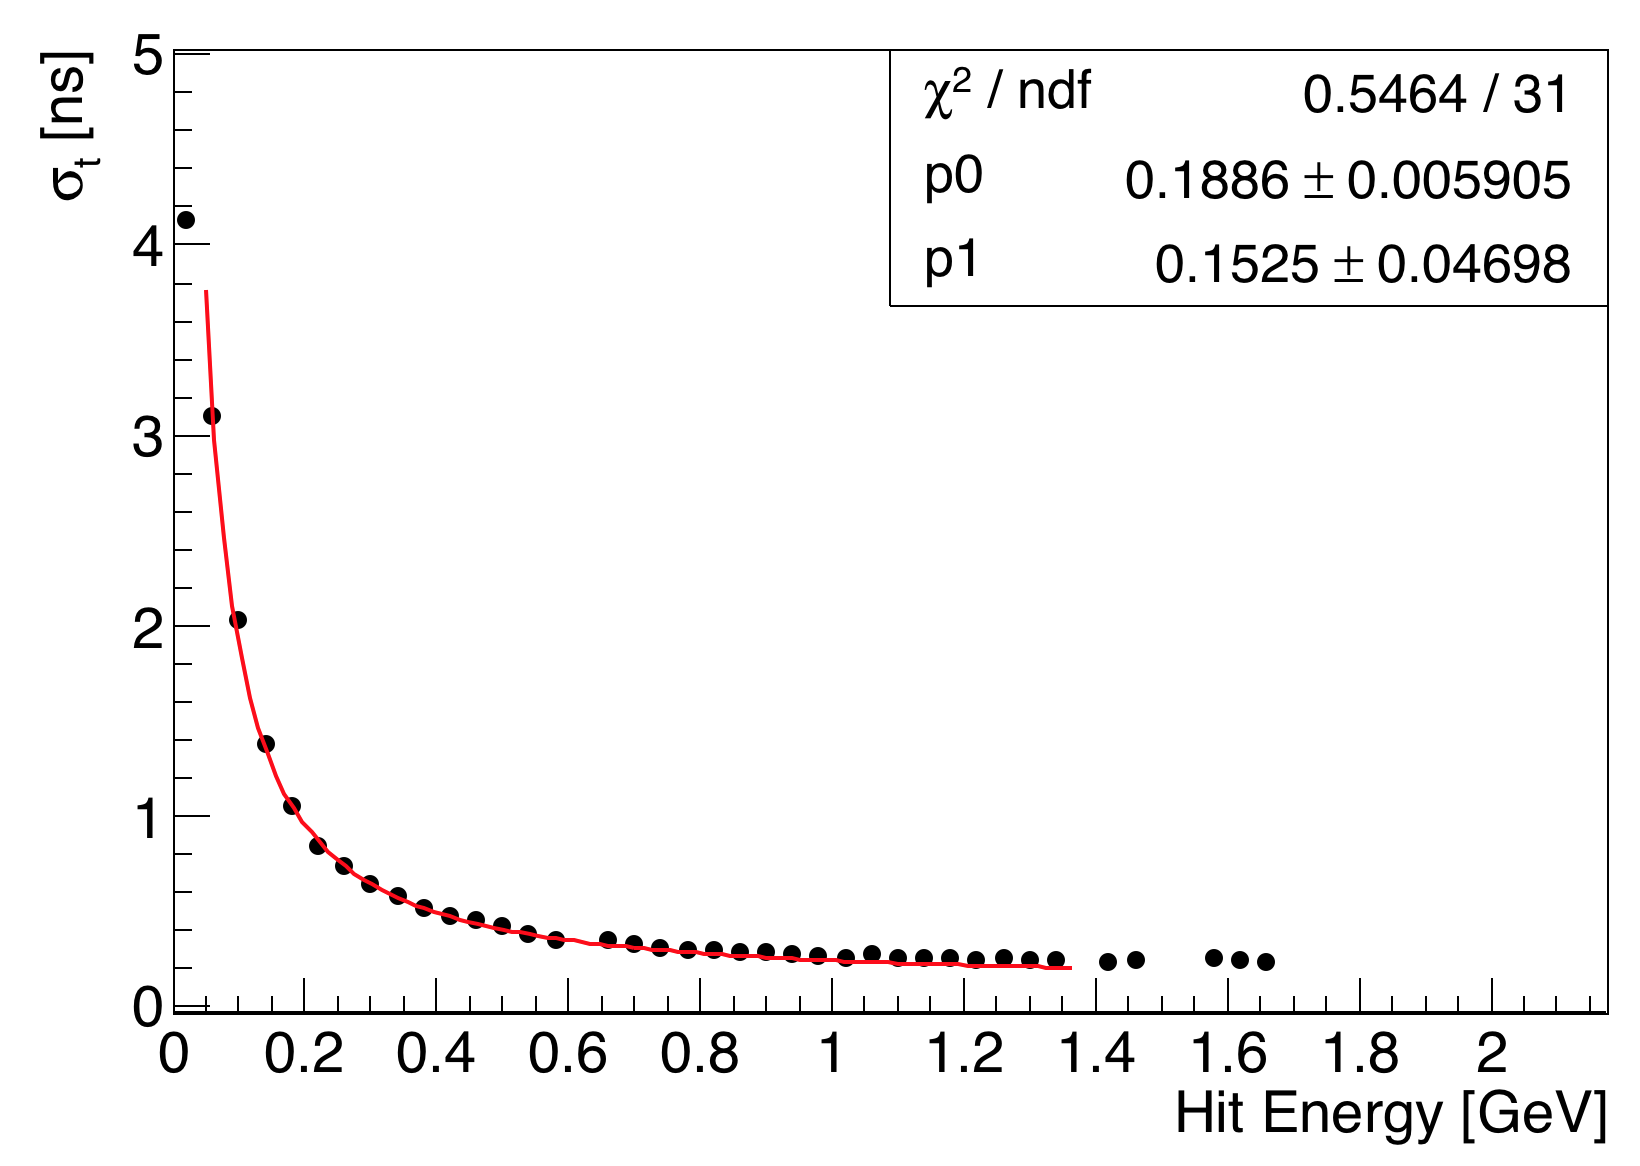
\includegraphics[width=0.6\textwidth]{pics/performance/timeRes2016.png}
  \caption[Time resolution of the ECal for the 2016 run ]{The time resolution as a function of energy is shown.}
  \label{Figure:timeRes}
\end{figure}

The time resolution as a function of hit energy shown in Figure~\ref{Figure:timeRes} is described by Equation~\eqref{Figure:twalkEqn}

\begin{equation}
	\label{eq:twalkEqn}
		\sigma_t \textsf{ [ns]} = \dfrac{p0}{E}\oplus p1	
\end{equation}

The measured time resolution for the time difference between two clusters is shown in Figure~\ref{Figure:timeRes2cl}.

\begin{figure}[H]
  \centering
      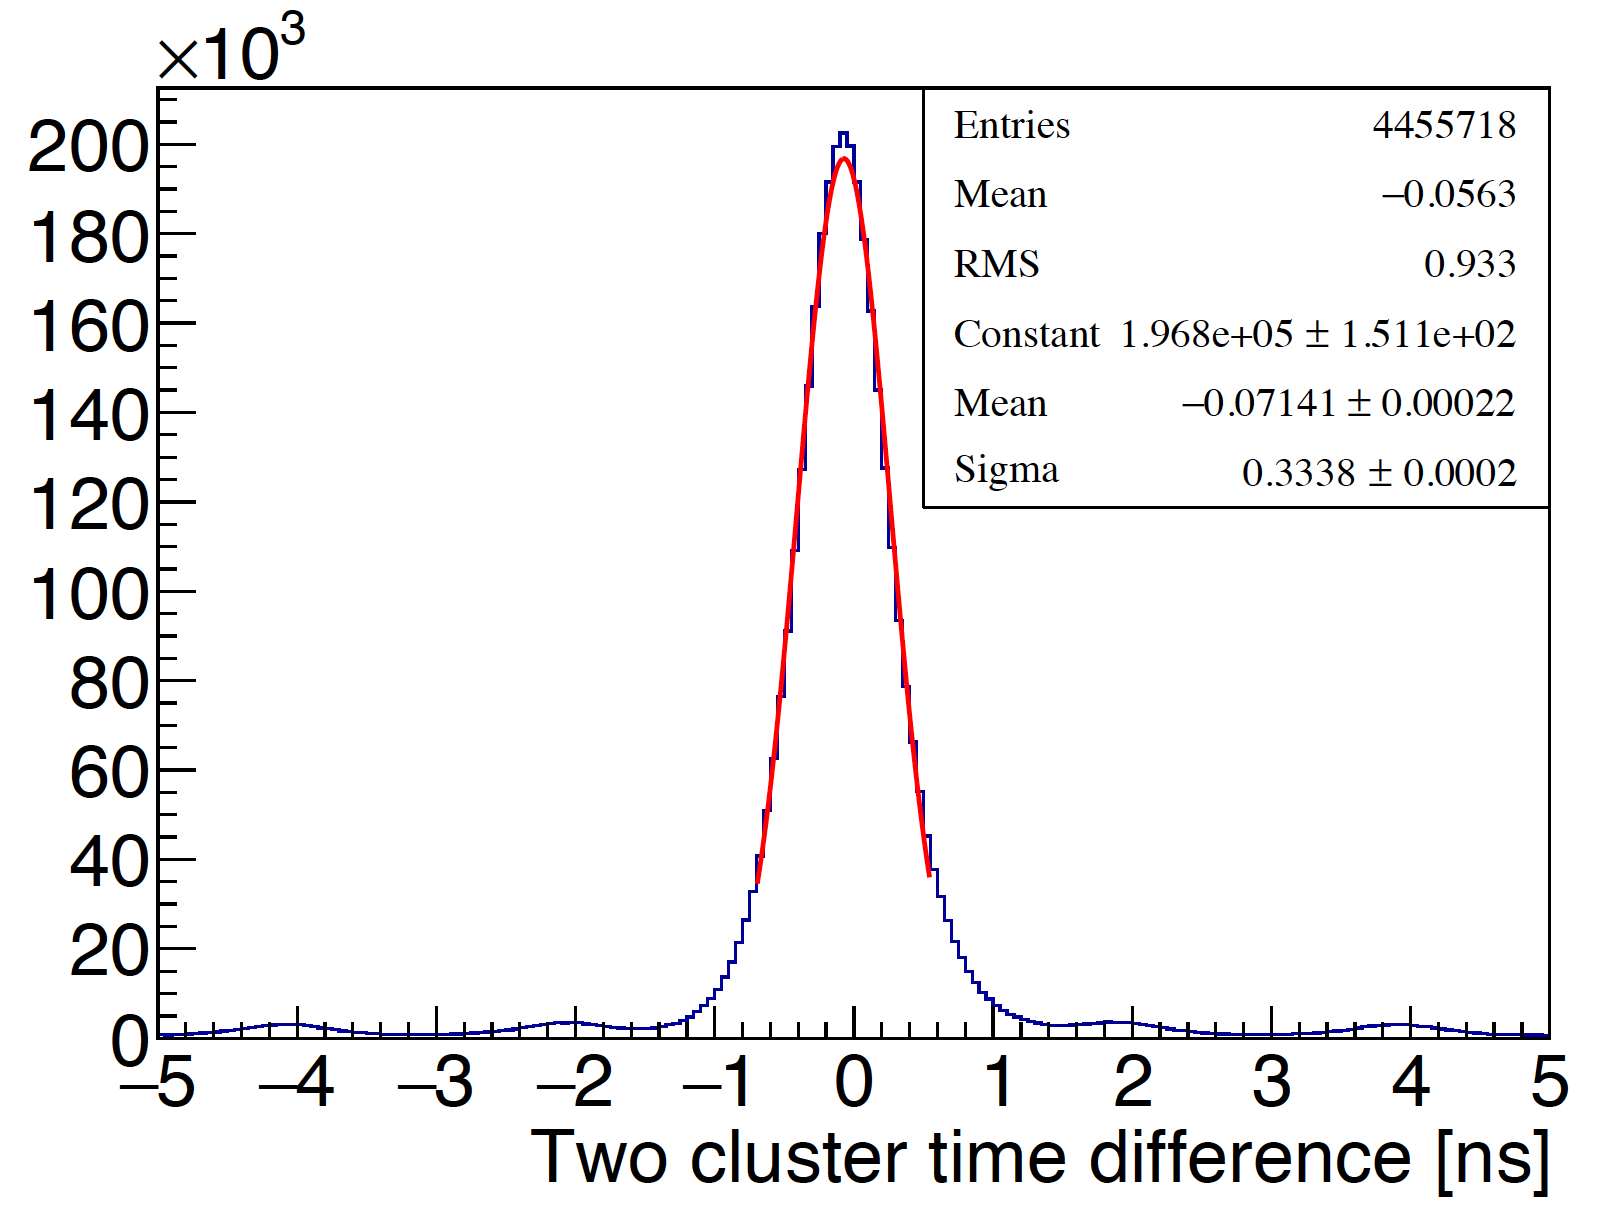
\includegraphics[width=0.6\textwidth]{pics/performance/2clusterTres.png}
  \caption[Time resolution for the time difference between two clusters]{The time difference between two clusters is shown. The energies sum to greater than 80$\%$ of the beam energy and have a resulting resolution of approximately 330~ps .}
  \label{Figure:timeRes2cl}
\end{figure}

As shown in Figure~\ref{Figure:timeRes2cl}, for two clusters that have an energy sum greater than 80$\%$ the beam energy in 2016, the resolution is approximately 330~ps. For the Engineering Run at a lower beam energy, the resolution of the time difference between two clusters was found to be approximately 470~ps. 